\subsubsection{Functional Requirements}
\begin{itemize}
  \item The user must provide a valid ID.
  \item The user must provide a valid password.
\end{itemize}

\subsubsection{Scenario 1}
Susan has just registered to PowerEnJoy and loads the home page in order to login, she then enters her credentials and submit the form. The credential are checked and Susan is redirected to the web application as a logged user.

\subsubsection{Scenario 2}
Mark is a typical PowerEnJoy user, he got used to the credentials form submission and types his password quickly. The password is not recognized by the system and Mark is asked to check his credentials. He then types more accurately and finally gets redirected to the web application. % todo: maybe forgot password

\subsubsection{Scenario 3}
A guest confused the login form with the registration one and after submiting the form is told that such user is not registered to the PowerEnJoy service. She then clicks on "Register to PowerEnJoy" and follows the registration procedure.


\subsubsection{Mockups}
\begin{figure}[!ht]
  \centering
  \vspace{0.2cm}
  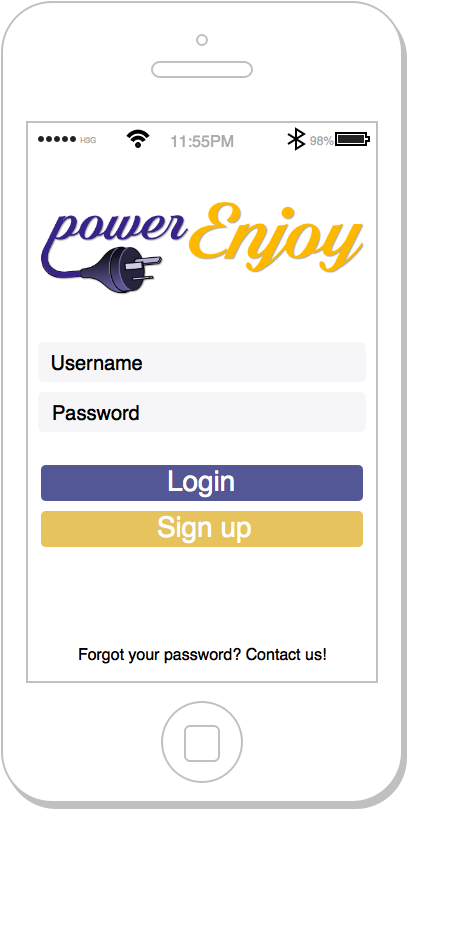
\includegraphics[width=0.25\textwidth]{/RASD/System_Functions/login_mockup}\\
  \vspace{0.4cm}
  %\caption{Mockup for the login mobile page} 
  \label{fig:login_mockup} 
\end{figure}
% maybe home page mockup here 


\subsubsection{Use-case table}
\begin{center}
  \begin{tabular}{ l | p{10cm} }
    \hline
    Actors & Guest\\ \hline
    Goal & G\ref{itm:goal-session}\\ \hline
    Entry conditions & The Guest is registered to PowerEnJoy and browse to the Log-in page in the web/mobile application. \\ \hline
    Flow of events &
\begin{itemize}
\item The Guest insert her \gls{ID} and \gls{pwd}.
\item The Guest clicks the Log-in button.
\item The system loads the User's homepage.
\end{itemize} \\ \hline
    Exit conditions & The User is in the PowerEnJoy homepage. \\ \hline
  Exceptions & 
\begin{itemize}
\item The Guest provides wrong username-password pair (the system signals a LoginError).
\item The Guest doesn't fill one of the fields (the systems signals an InformationLack).
\item The system is not able to complete the operation due to some internal issues or connection broken (the system signals a ConnectionFailure).
\end{itemize} \\ \hline
  \end{tabular}
\end{center}


\subsubsection{Sequence diagram}
\begin{figure}[!ht]
  \centering
  \vspace{0.1cm}
  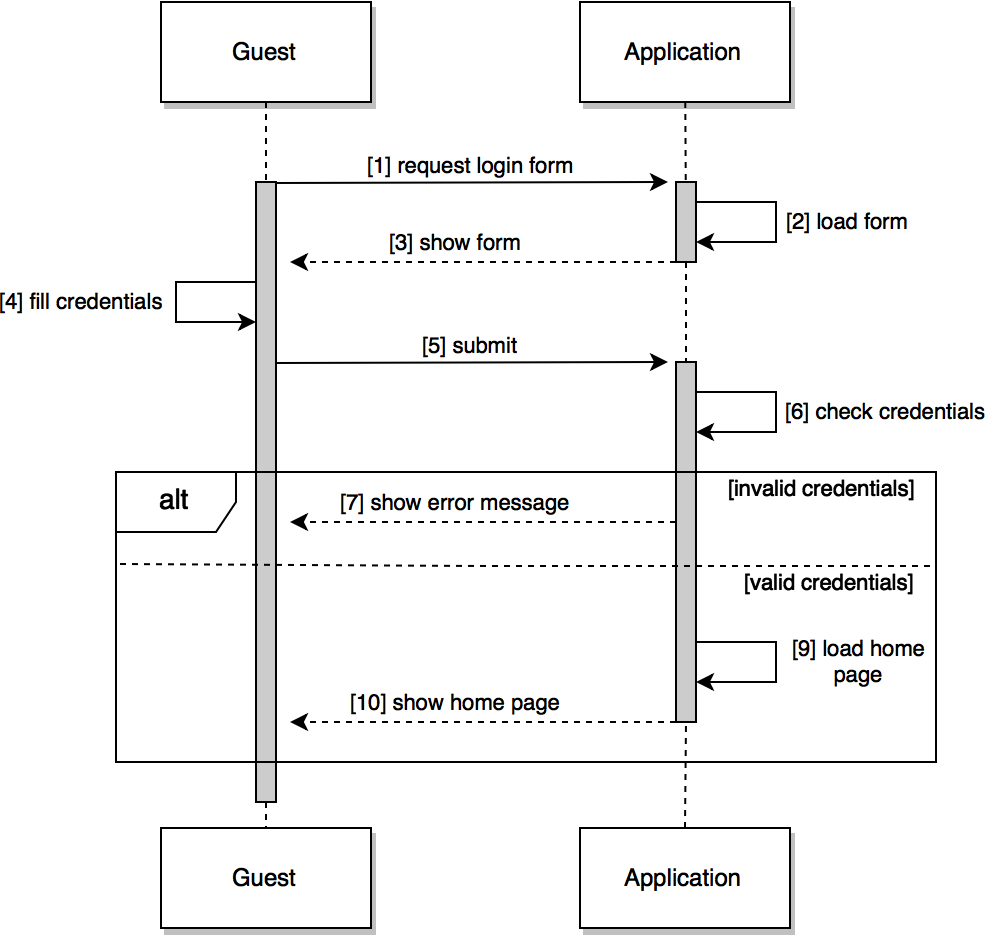
\includegraphics[width=0.6\textwidth]{/RASD/System_Functions/login_sequence}\\
  \vspace{0.1cm}
  %\caption{Sequence diagram for the login procedure} 
  \label{fig:login_sequence} 
\end{figure}

